\documentclass[conference]{IEEEtran}

\usepackage{cite}
\usepackage{amsmath}
\usepackage{amssymb}
\usepackage{url}
\usepackage{graphicx}
\usepackage{booktabs}
\usepackage{microtype}
\usepackage[table]{xcolor}
\usepackage{tikz}
\usetikzlibrary{positioning,arrows.meta,fit,backgrounds}
\usepackage{pgfplots}
\pgfplotsset{compat=1.18}
\usepgfplotslibrary{groupplots}
\usepackage[hidelinks]{hyperref}

\definecolor{phaseblue}{RGB}{52,152,219}
\definecolor{phasegreen}{RGB}{46,204,113}
\definecolor{phaseorange}{RGB}{230,126,34}
\definecolor{phasepurple}{RGB}{155,89,182}
\definecolor{phase1blue}{RGB}{52,152,219}
\definecolor{phase2green}{RGB}{46,204,113}
\definecolor{phase3orange}{RGB}{230,126,34}
\definecolor{phase4purple}{RGB}{155,89,182}
\definecolor{softgray}{RGB}{245,247,250}

\title{{\LARGE\textbf{Fairness-Aware Routing in Quantum Networks \& Clinical Settings}}\\
{\Large\textit{via Multi-Armed, Contextual, and Informative Bandit Methods}}\\[0.3em]
{\large\textit{(Rough Draft Report)}}}

\author{
\IEEEauthorblockN{Piter Z. Garcia}
\IEEEauthorblockA{MS Data Science / Decision-Making \& Algorithmic Fairness\\
Rochester Institute of Technology (RIT)\\
pizg8794@g.rit.edu}
\and
\IEEEauthorblockN{Daniel Krutz, Travis Desell}
\IEEEauthorblockA{Department of Software Engineering, Data Science\\
Rochester Institute of Technology (RIT)\\
dxkvse@g.rit.edu, tjdvse@g.rit.edu}
}

\begin{document}
\maketitle

\begin{abstract}
Sequential decision systems increasingly determine how scarce diagnostic,
computational, and communication resources are routed under uncertainty. This
project studies fairness-aware contextual multi-armed bandits for such
decisions when context is missing, delayed, noisy, or group-dependent. The
central claim is that clinical diagnostic decision workflows and quantum
network routing share the same structural failure mode: policies must choose
an action from partial feedback, yet the groups or flows with the least
reliable context can absorb the worst errors. The work develops a reusable
evaluation framework for non-contextual bandits, contextual bandits, and
informative contextual bandits across two executable environment families. The
quantum path reuses the legacy quantum-routing evaluation stack and saved-state
paths from the quantum-routing evaluation paper, while the clinical path now
runs through an embedded synthetic clinical environment with clinical models,
resource allocation, EQUITAS mediation, and governed fairness artifacts. Work
completed so far includes the related-work synthesis, domain model,
architecture specification, embedded clinical evaluator path, legacy quantum
fairness sidecar, default and fairness reporting datasets, validation-hub
artifacts, and CI-protected smoke gates. The contribution is a reproducible method for
measuring and mitigating time-evolving fairness disparities while
preserving utility under non-stationarity and limited context.
\end{abstract}

\section{Introduction}
Many applied data science systems are not one-shot predictors. They are
sequential decision systems that route limited resources under uncertainty:
which diagnostic test to order, which case to escalate, which model or
pipeline to trust, or which quantum-network path should receive scarce
entanglement-generation attempts. These decisions are difficult because the
system observes only partial feedback. The chosen action reveals an outcome,
but the unchosen alternatives remain counterfactual. They are also fairness
critical because the quality of the observed context is often uneven across
groups. When one population has delayed testing, incomplete patient history,
lower-quality measurements, or less representative calibration data, a policy
optimized only for aggregate reward can hide subgroup errors and compound
disparities over time.

This project frames that problem as fairness-aware contextual bandit learning.
At each round, a policy observes context, chooses an action, receives reward
only for the chosen action, and updates its future decisions. The scientific
question is not only whether contextual information improves reward, but
whether informative context and fairness-aware monitoring reduce disparities
when context is missing or degraded. This matters in clinical workflows because
false-negative or delayed-escalation gaps can produce direct harm. It also
matters in quantum-network routing because future communication systems will
allocate scarce probabilistic resources among competing flows; fairness in
success probability and latency is a service-quality issue rather
than a purely normative add-on.

The project uses two complementary environment families. The first is an
existing quantum-routing evaluation stack based on hybrid contextual bandits
for entanglement routing and qubit allocation~\cite{garcia2026threat_aware_quantum_routing}.
That stack already exposes uncertainty, adversarial or non-stationary
conditions, legacy testbed conventions, and stateful evaluator artifacts. The
second is an embedded clinical simulation motivated by equitable bioinformatics
and fairness auditing work~\cite{garcia2025equitable_bioinformatics}. The
clinical environment models the routing of scarce tests, retesting capacity,
escalation decisions, diagnostic attention, and model-assisted triage across
sites and cohorts. Under volatile conditions such as a pandemic, threat,
demand, evidence quality, and resource availability can change rapidly; this
makes the clinical routing setting structurally comparable to quantum routing
under noisy links, uncertain entanglement generation, and non-stationary
service conditions. The two-domain design tests whether fairness mechanisms
and policy-update strategies transfer across fundamentally different
applications with the same partial-feedback allocation structure.

The current rough draft reports the mostly completed design and implementation
foundation rather than final experimental results. The remainder of the paper
is organized as follows. Section~II summarizes related work. Section~III
describes the methodology and domain model. Section~IV describes the
implementation and reproducibility architecture. Section~V summarizes the data
sets and experimental inputs. Section~VI gives preliminary validation evidence.
Sections~VII and VIII describe future work and conclusions.

This rough draft does not claim that the final fairness results are complete.
Instead, it consolidates the work into a single preliminary
final-paper structure. That consolidation is important because the project is
cross-domain. The organizing idea used throughout this draft is
that both domains are sequential routing systems whose fairness risk emerges
from unequal context quality. The clinical system routes diagnostic attention;
the quantum system routes probabilistic network resources. Both require
learning under partial feedback, non-stationarity, and subgroup- or flow-level
performance monitoring.

\section{Related Work}
\subsection{Bandits and Contextual Sequential Decision-Making}
Multi-armed bandits model online learning under partial feedback, balancing
exploration and exploitation while observing rewards only for selected
actions. UCB-style algorithms provide finite-time regret guarantees in
stochastic settings~\cite{auer2002finite}, while Thompson sampling offers a
Bayesian alternative that often performs well empirically~\cite{russo2018tutorial}.
The broader bandit literature provides the regret and uncertainty-estimation
foundation for this project~\cite{lattimore2020bandit}. Contextual bandits
extend this model by conditioning action choice on observed side information.
LinUCB and related methods demonstrate how context can improve online
personalization and decision quality~\cite{li2010contextual,abbasi2011linear},
and reduction-based contextual bandit approaches show how richer policy
classes can be scaled~\cite{agarwal2014taming}. However, most of this work
optimizes expected reward and assumes that context is observed correctly or
representatively.

Offline policy evaluation is also relevant because the final framework will
compare policies from logged simulator outputs as well as from fresh online
runs. Doubly robust estimators combine reward modeling with inverse-propensity
weighting and can reduce variance when evaluating bandit policies from logged
data~\cite{dudik2011doubly}. In this project, those ideas motivate careful
logging of actions, propensities or selection rules, context snapshots, and
oracle comparisons. They also highlight a fairness concern: if one group has
less support in the logged data, group-specific estimates can be noisier even
when the aggregate estimator appears stable.

\subsection{Fairness, Missing Context, and Non-Stationarity}
Fairness in supervised learning is often expressed through group-conditioned
error criteria such as equality of opportunity and equalized odds
\cite{hardt2016equality}. In sequential settings, the problem is harder:
fairness constraints affect exploration, data collection, and the future
evidence available to the learner. Joseph et al. connect fairness to bandit
learning directly~\cite{joseph2016fairness}, while Chen et al. study fair
contextual multi-armed bandits with explicit group constraints
\cite{chen2020fair}. Offline contextual-bandit fairness work shows how
importance-weighted estimators can support high-probability constraints
\cite{metevier2019offline}, but online distribution shift and time-evolving
disparity remain open practical challenges. Non-stationary bandit work
addresses changing reward distributions through discounting, change detection,
or variation budgets~\cite{garivier2008ucb,besbes2014stochastic}. Limited or
unobserved context work similarly motivates algorithms that remain robust when
features are unavailable or latent~\cite{bouneffouf2017context,park2022efficient}.

The limitation across these areas is that they often address only one axis of
the final problem. Standard bandits provide regret machinery but not fairness
audits. Fairness definitions clarify what disparities matter but are often
studied in static supervised settings. Non-stationary bandits handle changing
reward processes but usually report aggregate utility. Restricted-context work
handles missing features but rarely treats missingness as a group-dependent
fairness mechanism. The present project combines these axes by treating
missing context, time-varying reward, and group disparity as simultaneous
properties of the same learning process.

\subsection{Clinical Fairness and Quantum Routing}
Clinical algorithmic bias studies show that proxy targets and measurement
processes can encode structural inequities, producing under-allocation for
some groups even when aggregate performance appears strong~\cite{obermeyer2019dissecting}.
This motivates outcome-based disparity monitoring such as false-negative and
false-positive gaps. In parallel, quantum-network research describes an
emerging communication infrastructure in which routing decisions are governed
by probabilistic entanglement generation, fidelity, storage limits, and
scarce resources~\cite{wehner2018quantum,pant2019routing,caleffi2017optimal}.
Prior quantum routing work usually emphasizes throughput, fidelity, or
robustness rather than group-based service equity. The gap this project
addresses is therefore the intersection of contextual bandit learning,
missing context, non-stationarity, and explicit fairness monitoring across
both clinical and quantum-resource routing domains.

\begin{table}[t]
\caption{How the reviewed literature supports the project.}
\label{tab:related_map}
\centering
\small
\begin{tabular}{p{0.29\columnwidth}p{0.65\columnwidth}}
\toprule
\textbf{Literature area} & \textbf{Role in this rough draft} \\
\midrule
Bandit foundations & partial feedback, regret \& baselines \\
Contextual bandits & model side data \& missing-context sensitivity \\
Fairness definitions & outcome gaps, FNR/FPR \& service equity \\
Non-stationarity & shift scenarios \& time-based disparity curves \\
Clinical bias studies & subgroup error monitor \& proxy-risk caution \\
Quantum routing & resource-scarce routing testbed \& stateful simulator \\
\bottomrule
\end{tabular}
\end{table}

Table~\ref{tab:related_map} summarizes the role of each category. The final
paper will expand this discussion with direct comparisons once the final
experiments are complete, but the rough draft already establishes the
scientific gap: existing work rarely evaluates outcome-based fairness under
missing context and distribution shift across two structurally similar but
domain-distinct routing systems.

\section{Approach and Methodology}
\subsection{Shared Missing-Context Routing Model}
The methodology treats both domains as routing under missing context. Business
Understanding identifies the shared harm mechanism: clinical and quantum
systems route scarce resources under uncertainty, and unequal context quality
can produce repeated allocation harm. Data Understanding identifies the
measurable patterns that make that harm testable, including group, site,
cohort, service line, test distribution, escalation action, latency, reward,
success, scenario, allocator, route choice, and evaluator-state fields.

In the clinical domain, the routed resource is diagnostic attention: scarce
tests, retests, triage escalation, model-assisted prioritization, or
model/pipeline selection. In the quantum domain, the routed resource is
entanglement-generation effort, qubit allocation, or path capacity. In both
domains, the policy observes partial context, chooses an action, receives
partial feedback, and updates. The key experimental variable is the richness
and reliability of context available to the policy.

\begin{figure*}[t]
\centering
\resizebox{0.97\textwidth}{!}{%
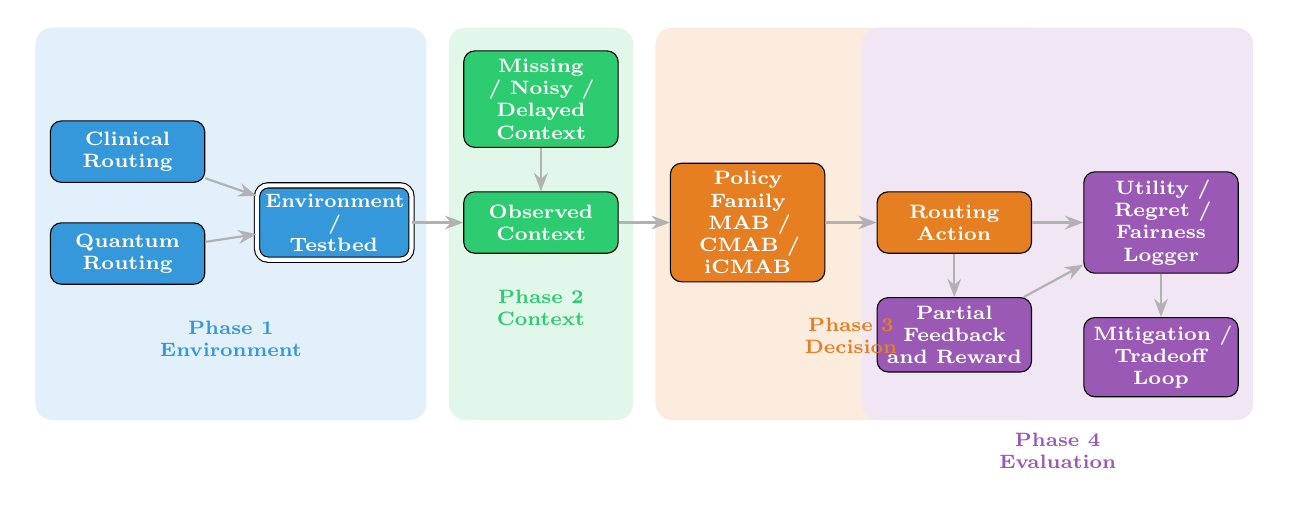
\begin{tikzpicture}[
  font=\scriptsize,
  box/.style={draw, rounded corners=4pt, align=center,
              text width=1.75cm, minimum height=0.78cm,
              inner sep=3pt, text=white, font=\scriptsize\bfseries},
  phase1/.style={box, fill=phase1blue},
  phase2/.style={box, fill=phase2green},
  phase3/.style={box, fill=phase3orange},
  phase4/.style={box, fill=phase4purple},
  arr/.style={-Stealth, thick, gray!60},
  lbl/.style={font=\scriptsize\bfseries, align=center}
]
\node[phase1] (clin)  {Clinical\\Routing};
\node[phase1, below=0.5cm of clin]  (quant) {Quantum\\Routing};
\node[phase1, right=0.65cm of clin, yshift=-0.9cm,
      double, double distance=1.5pt] (env) {Environment /\\Testbed};
\node[phase2, right=0.65cm of env]  (ctx) {Observed\\Context};
\node[phase2, above=0.55cm of ctx]  (deg) {Missing / Noisy /\\Delayed Context};
\node[phase3, right=0.65cm of ctx]  (pol) {Policy Family\\MAB / CMAB / iCMAB};
\node[phase3, right=0.65cm of pol]  (act) {Routing\\Action};
\node[phase4, below=0.55cm of act]  (fb)  {Partial Feedback\\and Reward};
\node[phase4, right=0.65cm of act]  (log) {Utility / Regret /\\Fairness Logger};
\node[phase4, below=0.55cm of log]  (mit) {Mitigation /\\Tradeoff Loop};

\draw[arr] (clin)--(env); \draw[arr] (quant)--(env);
\draw[arr] (env)--(ctx);  \draw[arr] (deg)--(ctx);
\draw[arr] (ctx)--(pol);  \draw[arr] (pol)--(act);
\draw[arr] (act)--(fb);   \draw[arr] (act)--(log);
\draw[arr] (fb)--(log);   \draw[arr] (log)--(mit);

\begin{pgfonlayer}{background}
  \node[inner sep=8pt,
        fit=(clin)(quant)(env)(ctx)(deg)(pol)(act)(fb)(log)(mit)] (all) {};
  \node[inner sep=5pt, fit=(clin)(quant)(env)] (bg1) {};
  \node[inner sep=5pt, fit=(ctx)(deg)]         (bg2) {};
  \node[inner sep=5pt, fit=(pol)(act)]         (bg3) {};
  \node[inner sep=5pt, fit=(fb)(log)(mit)]     (bg4) {};
  \fill[phase1blue!15,   rounded corners=6pt]
      (bg1.west |- all.north) rectangle (bg1.east |- all.south);
  \fill[phase2green!15,  rounded corners=6pt]
      (bg2.west |- all.north) rectangle (bg2.east |- all.south);
  \fill[phase3orange!15, rounded corners=6pt]
      (bg3.west |- all.north) rectangle (bg3.east |- all.south);
  \fill[phase4purple!15, rounded corners=6pt]
      (bg4.west |- all.north) rectangle (bg4.east |- all.south);
\end{pgfonlayer}

\node[lbl, text=phase1blue,   below=0.15cm of bg1] {\textbf{Phase 1}\\Environment};
\node[lbl, text=phase2green,  below=0.15cm of bg2] {\textbf{Phase 2}\\Context};
\node[lbl, text=phase3orange, below=0.15cm of bg3] {\textbf{Phase 3}\\Decision};
\node[lbl, text=phase4purple, below=0.15cm of bg4] {\textbf{Phase 4}\\Evaluation};
\end{tikzpicture}}
\vspace{0.4em}
\resizebox{0.97\textwidth}{!}{%
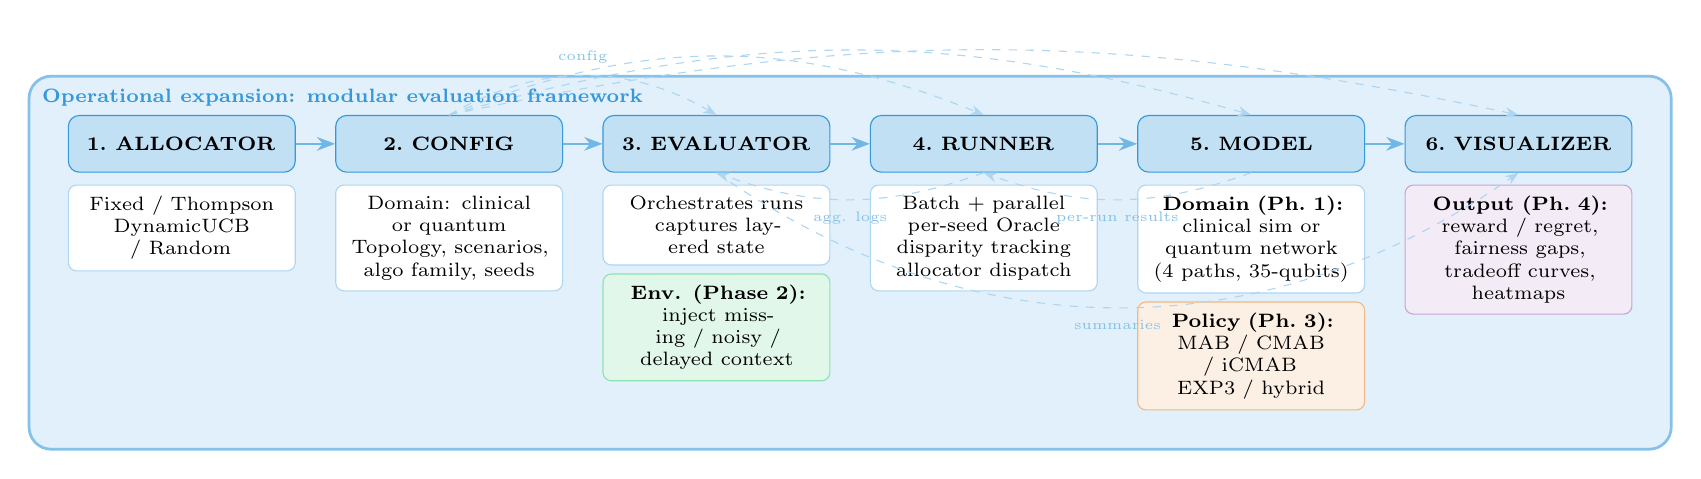
\begin{tikzpicture}[
  font=\scriptsize,
  mod/.style={rectangle, draw=phase1blue, rounded corners=4pt, align=center,
              text width=2.6cm, minimum height=0.72cm,
              inner sep=4pt, font=\scriptsize\bfseries,
              fill=phase1blue!30},
  det/.style={rectangle, draw=phase1blue!40, rounded corners=3pt, align=center,
              text width=2.6cm, inner sep=4pt, font=\scriptsize, fill=white},
  det2/.style={det, fill=phase2green!15,  draw=phase2green!55},
  det3/.style={det, fill=phase3orange!12, draw=phase3orange!55},
  det4/.style={det, fill=phase4purple!12, draw=phase4purple!55},
  arr/.style={-Stealth, thick, phase1blue!70},
  darr/.style={-Stealth, dashed, phase1blue!40},
  lbl/.style={font=\tiny, align=center, text=phase1blue!60}
]
\node[mod] (A) {1.~ALLOCATOR};
\node[det, below=0.15cm of A] (Ad) {Fixed / Thompson\\DynamicUCB / Random};
\node[mod, right=0.5cm of A] (C) {2.~CONFIG};
\node[det, below=0.15cm of C] (Cd) {Domain: clinical\\or quantum\\Topology, scenarios,\\algo family, seeds};
\node[mod, right=0.5cm of C] (E) {3.~EVALUATOR};
\node[det, below=0.15cm of E] (Ed) {Orchestrates runs\\captures layered state};
\node[det2, below=0.1cm of Ed] (Env) {\textbf{Env. (Phase~2):}\\inject missing / noisy /\\delayed context};
\node[mod, right=0.5cm of E] (R) {4.~RUNNER};
\node[det, below=0.15cm of R] (Rd) {Batch + parallel\\per-seed Oracle\\disparity tracking\\allocator dispatch};
\node[mod, right=0.5cm of R] (M) {5.~MODEL};
\node[det, below=0.15cm of M] (Md) {\textbf{Domain (Ph.~1):}\\clinical sim or\\quantum network\\(4 paths, 35-qubits)};
\node[det3, below=0.1cm of Md] (Alg) {\textbf{Policy (Ph.~3):}\\MAB / CMAB / iCMAB\\EXP3 / hybrid};
\node[mod, right=0.5cm of M] (V) {6.~VISUALIZER};
\node[det4, below=0.15cm of V] (Vd) {\textbf{Output (Ph.~4):}\\reward / regret,\\fairness gaps,\\tradeoff curves,\\heatmaps};
\draw[arr] (A)--(C); \draw[arr] (C)--(E);
\draw[arr] (E)--(R); \draw[arr] (R)--(M); \draw[arr] (M)--(V);
\draw[darr] (C.north) to[bend left=30] node[lbl,above=1pt]{config} (E.north);
\draw[darr] (C.north) to[bend left=22] (R.north);
\draw[darr] (C.north) to[bend left=16] (M.north);
\draw[darr] (C.north) to[bend left=12] (V.north);
\draw[darr] (M.south) to[bend left=20] node[lbl,below=1pt]{per-run results} (R.south);
\draw[darr] (R.south) to[bend left=20] node[lbl,below=1pt]{agg. logs} (E.south);
\draw[darr] (E.south) to[bend right=35] node[lbl,below=1pt]{summaries} (V.south);
\begin{pgfonlayer}{background}
  \node[inner sep=14pt, rounded corners=8pt,
        fill=phase1blue!15, draw=phase1blue!60, line width=1pt,
        fit=(A)(Ad)(C)(Cd)(E)(Ed)(Env)(R)(Rd)(M)(Md)(Alg)(V)(Vd)] (bbox) {};
\end{pgfonlayer}
\node[anchor=north west, inner sep=5pt, font=\scriptsize\bfseries, text=phase1blue]
  at (bbox.north west) {\textbf{Operational expansion: modular evaluation framework}};
\end{tikzpicture}}
\caption{Shared domain model and operational evaluation framework. The top panel isolates the causal chain that can generate unfair outcomes in both domains: the environment defines the routing problem, missing/noisy/delayed information perturbs only the context stage, the policy family acts on the degraded observation, and utility--fairness logging plus mitigation occur only after partial feedback is received. Clinical actions map to test ordering, retesting, or escalation; quantum actions map to route or allocator decisions. The bottom panel expands the implementation stack and highlights the three experimental intervention points used throughout the project: context degradation in the evaluator environment, policy-family choice in the model layer, and utility--fairness tradeoff analysis in the visualizer.}
\label{fig:domain_model}
\end{figure*}

Figure~\ref{fig:domain_model} summarizes the shared model. Phase 1 defines
the environment and available resources. Phase 2 determines what context is
observed and which context is missing or degraded. Phase 3 selects an action
using a non-contextual, contextual, or informative contextual bandit policy.
Phase 4 evaluates both performance and fairness, then feeds mitigation or
updated policy information back into future decisions. This model is useful
because it makes the failure point explicit: if context is systematically
lower-quality for one group or flow class, the learning process can convert
measurement inequity into repeated allocation inequity. It also clarifies where
the experiments intervene: missingness is injected before the policy sees the
state, while mitigation is evaluated only after utility and disparity have been
logged.

At round $t$, the learner receives an observed context vector
$\tilde{\mathbf{x}}_t$, which may differ from the latent complete context
$\mathbf{x}_t$ because of missingness, delay, or measurement noise. It chooses
an action $a_t$ and observes reward $r_t(a_t)$ only for that action. Utility is
tracked through cumulative regret,
\begin{equation}
R_T = \sum_{t=1}^{T} \left(r_t(a_t^*) - r_t(a_t)\right),
\label{eq:regret}
\end{equation}
where $a_t^*$ is the best available action under the simulator oracle.
Fairness is tracked through time-indexed disparity gaps,
\begin{equation}
\Delta_m(t) =
\left|m_t(G=0) - m_t(G=1)\right|,
\label{eq:gap}
\end{equation}
where $m_t$ is a domain-specific outcome metric such as false-negative rate,
success probability, latency, or escalation delay. This notation separates the
learning objective from the fairness audit: a policy can have low regret in
aggregate while still producing high $\Delta_m(t)$ for specific groups.

\subsection{Design Decisions}
Bandits are used instead of full reinforcement learning because both testbeds
provide bandit feedback: only the chosen diagnostic or routing action reveals
an outcome. The project compares three policy families. Non-contextual MABs
serve as a baseline for action-only learning. Contextual bandits test whether
observed context improves utility and equity. Informative contextual bandits
represent policies that recover, augment, or better weight missing context.
The simulation-first clinical design avoids sensitive patient data while
allowing controlled missingness and group-specific measurement noise. The
quantum testbed reuses an existing, domain-grounded routing environment so
that fairness analysis is built on top of realistic uncertainty rather than
a toy network.

Fairness is measured as an online outcome property. In diagnostics, the target
metrics are group-wise false-negative and false-positive gaps, along with
utility and cost-sensitive reward. In quantum routing, service equity is
measured through success-probability and latency gaps across flow groups.
Mitigation mechanisms under consideration include fairness-regularized policy
updates, group-aware calibration or thresholding, and missingness-aware
context augmentation. These mechanisms will be evaluated as tradeoffs rather
than as free improvements, because fairness constraints can reduce short-term
reward while improving reliability and equity.

\subsection{Experimental Questions}
The final experiments will answer four questions. First, how much does context
improve utility and fairness relative to non-contextual baselines when all
groups have comparable context quality? Second, how quickly do fairness gaps
emerge when one group or flow class receives noisier, delayed, or incomplete
context? Third, do missingness-aware or fairness-regularized policy updates
reduce outcome disparities without unacceptable utility loss? Fourth, do the
same policy-update strategies transfer between clinical diagnostic simulation
and quantum routing, or are the fairness mechanisms domain-specific? These
questions define the planned analysis tables and figures: reward/regret curves,
time-evolving disparity curves, mitigation tradeoff plots, and cross-domain
transfer summaries.

\subsection{Planned Mitigation Strategy}
The first mitigation family will treat fairness as a penalty or constraint in
the policy-update loop. In the simplest form, the learner receives a utility
reward and a disparity signal; policy updates are then adjusted when recent
group-specific outcomes exceed an allowed gap. This makes fairness operational
during learning instead of applying it only after the experiment. A second
family will use missingness-aware context augmentation. If a group or flow class
systematically receives incomplete context, the policy can either acquire
additional features, impute missing indicators, or adjust confidence estimates
so that uncertainty caused by measurement gaps is not mistaken for low expected
value. A third family will test group-aware calibration or thresholding at the
decision boundary. This is especially relevant for diagnostic-like escalation,
where a small threshold shift can change false-negative rates.

The mitigation comparison will be conservative. The final paper will not claim
that lower disparity is automatically better if the policy produces unsafe or
unusable utility loss. Instead, each mitigation will be evaluated through
utility--fairness tradeoff curves. The preferred policy is expected to be one
that preserves most of the utility of contextual learning while reducing
time-evolving disparity under missing context. This is why the project compares
MAB, CMAB, and iCMAB policies under the same seeds, scenario settings, and
logged artifacts: the point is to isolate the effect of context quality and
fairness-aware updates rather than confounding algorithm choice with simulator
configuration.

\section{Implementation and Reproducibility}
\subsection{Execution Paths}
The implementation is designed around reproducibility. The quantum side uses
three execution paths inherited from the upstream quantum project: notebooks
for fast interactive replication, a local environment for development and
testing, and GCP/batch scripts for longer runs. The notebook and local paths
support the legacy quantum testbeds and saved-state conventions documented in
the quantum-routing evaluation paper~\cite{garcia2026threat_aware_quantum_routing}.
The clinical side now runs through an embedded evaluator path consisting of
\texttt{ClinicalExperimentEvaluator}, \texttt{ClinicalExperimentRunner},
\texttt{ClinicalEnvironment}, clinical resource allocation, clinical model
objects, and EQUITAS mediation. The local path uses a virtual environment,
dependencies from \texttt{requirements.txt}, and validation scripts. The GCP
path uses startup and dynamic-runner scripts for larger allocator and
time-scale experiments.

\begin{table}[t]
\caption{Implementation layers and the role of reproducibility.}
\label{tab:implementation}
\centering
\small
\begin{tabular}{p{0.32\columnwidth}p{0.65\columnwidth}}
\toprule
\textbf{Layer} & \textbf{Role} \\
\midrule
Configuration & fixed seeds, settings, run scales \& output roots \\
Collection/state access & retrieves Drive framework \& model states \\
Runner/allocator & executes routing actions \& qubit allocation \\
Evaluator & winners, reward, efficiency, \& gap summaries \\
Visualizer/analysis & plots, summaries \& review-facing tables \\
CRISP+ML package & a deterministic pipeline, tests \& merge checks \\
\bottomrule
\end{tabular}
\end{table}

Table~\ref{tab:implementation} summarizes the software entities. The quantum
workflow relies on evaluator and runner objects that save framework state,
model state, and analysis outputs. These state layers support interruption
recovery and replication. The CRISP+ML package in its own repository is
a reviewer-safe implementation harness that mirrors the project methodology:
data collection, cleaning, preparation, exploration, mining, evaluation, and
postprocessing. It exposes command-line stages through \texttt{python -m
experiments}, writes deterministic artifacts under a result directory, and
records provenance through a pipeline manifest.

The state design is intentionally layered. Individual models can save model
state so interrupted algorithm runs do not always require recomputation.
Experiment runners can save complete experiment state so a particular
scenario, seed, allocator, and capacity setting can be resumed. Evaluators can
save scenario-level collections of runner outputs so a full comparison can be
extended, summarized, or audited later. This layered persistence is important
for research validity because long-running quantum-routing jobs can be
interrupted, and because later fairness analysis may need to reconstruct how a
specific result was produced. In the final system, allocator-runner state will
become a fourth layer that aggregates all evaluator runs for a specific
allocator and supports broader cross-scenario analysis.

\begin{table}[t]
\caption{CRISP+ML mapping used by the reviewer-safe implementation.}
\label{tab:crisp}
\centering
\small
\begin{tabular}{p{0.24\columnwidth}p{0.67\columnwidth}}
\toprule
\textbf{Lifecycle stage} & \textbf{Concrete artifact} \\
\midrule
Data collection & synthetic fairness-style raw records \& metadata \\
Data cleaning & validated, normalized data \& context handling \\
Data preparation & train/test artifacts \& model-ready feature table \\
Data exploration & summary statistics \& group/context diagnostics \\
Data mining & light deterministic model/bandit-style run \\
Evaluation & utility metrics and group-disparity summaries \\
Presentation & final table, manifest, and visualization artifact \\
\bottomrule
\end{tabular}
\end{table}

Table~\ref{tab:crisp} shows how the small code package maps to a recognized
methodology rather than an ad hoc script sequence. The same conceptual
pipeline will be used for the final experiments: collect or generate simulator
records, clean and validate them, prepare model-ready contexts, run policy
families, evaluate utility and fairness, and present results in reproducible
plots and tables.

\subsection{Code Review and Validation Path}
The code artifact is intentionally object-oriented. A base pipeline-stage
interface defines the stage contract, concrete classes implement each CRISP+ML
phase, typed configuration and artifact containers carry paths and metadata,
and a pipeline orchestrator runs stages end-to-end or stage-by-stage. Unit
tests validate each stage and the overall manifest. The merge-check command
runs the full quick-review pipeline and the unit-test suite, giving reviewers
a fast way to verify that the repository executes before inspecting the larger
quantum workflow. This design supports the rough-draft requirement that
another party should be able to recreate the system or software from the
description.

The package also supports stage-level commands rather than requiring reviewers
to run notebooks. Each stage can be executed independently, and the full
pipeline command composes those same objects. This separation makes failures
diagnosable: a schema error should fail in cleaning, a feature construction
problem should fail in preparation, and a missing metric should fail in
evaluation. The GitHub merge-check workflow mirrors the local validation path,
so code submitted for review is checked against the same unit tests and
quick-run pipeline that a reviewer would execute manually.

\begin{figure*}[t]
\centering
\resizebox{0.98\textwidth}{!}{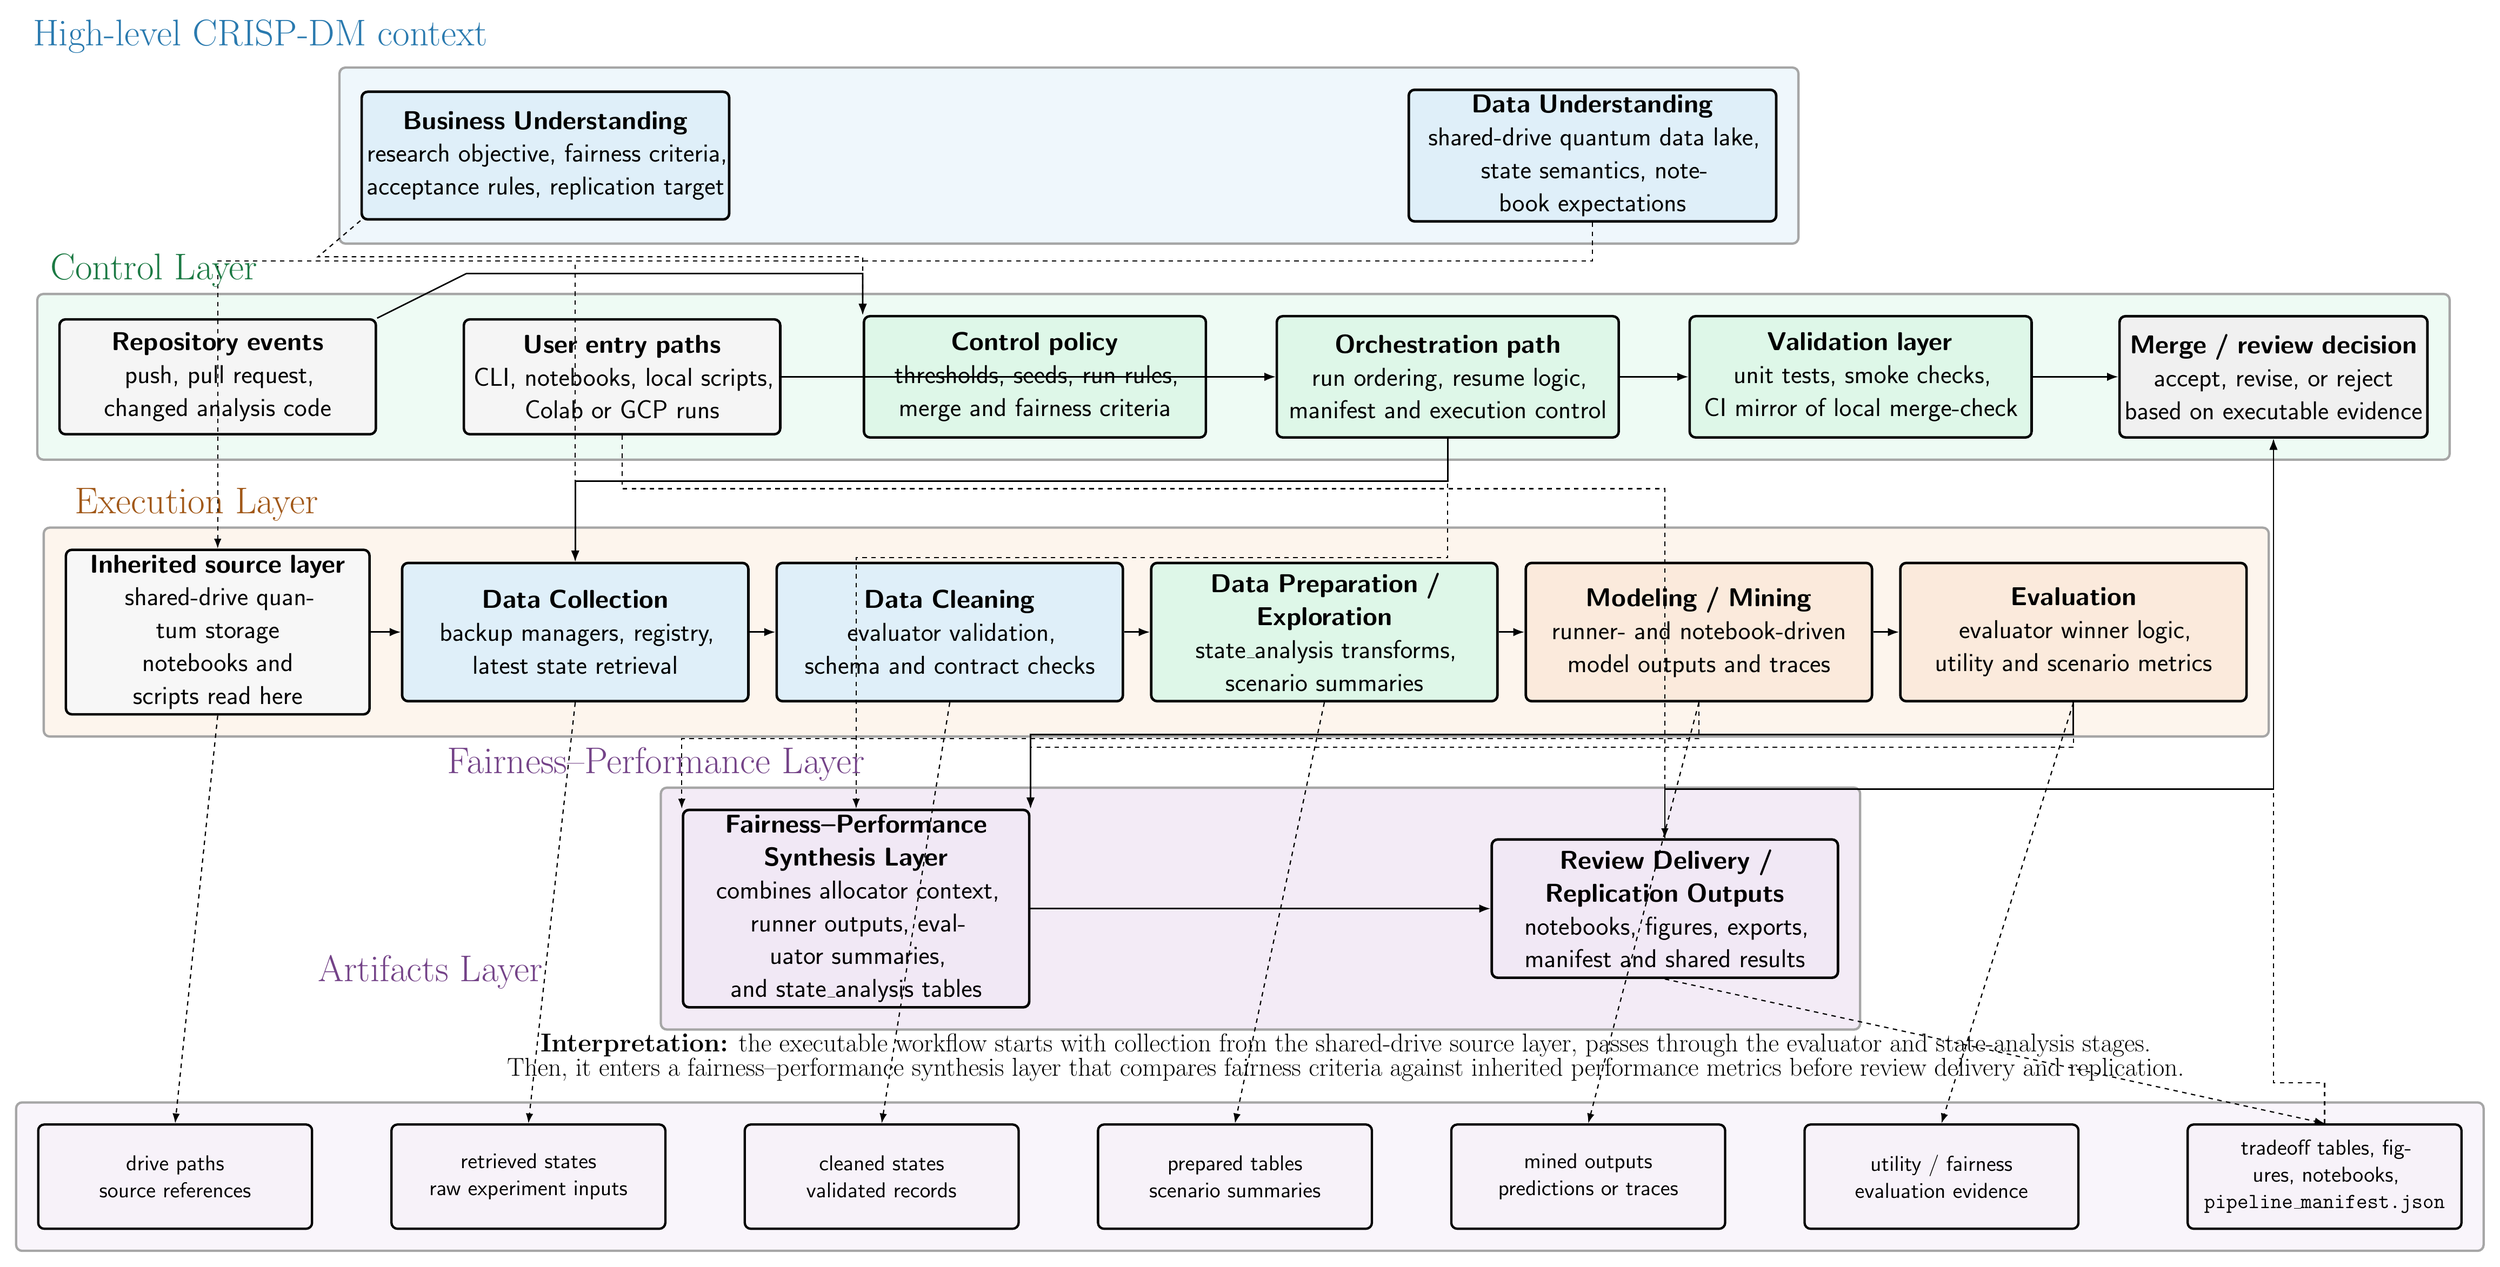
\begin{tikzpicture}[
font=\sffamily\Large,>=Latex,
layerband/.style={rectangle,rounded corners,inner sep=14pt,line width=1.55pt,draw=black!35},
event/.style={rectangle,draw=black,rounded corners,minimum height=2.70cm,text width=7.2cm,align=center,fill=gray!8,line width=1.65pt,font=\sffamily\LARGE},
control/.style={rectangle,draw=black,rounded corners,minimum height=2.85cm,text width=7.8cm,align=center,line width=1.65pt,font=\sffamily\LARGE},
context/.style={rectangle,draw=black,rounded corners,minimum height=3.00cm,text width=8.4cm,align=center,line width=1.7pt,font=\sffamily\LARGE},
stage/.style={rectangle,draw=black,rounded corners,minimum height=3.25cm,text width=7.9cm,align=center,line width=1.7pt,font=\sffamily\LARGE},
sourcebox/.style={rectangle,draw=black,rounded corners,minimum height=2.70cm,text width=6.9cm,align=center,fill=gray!6,line width=1.65pt,font=\sffamily\LARGE},
artifact/.style={rectangle,draw=black,rounded corners,minimum height=2.45cm,text width=6.2cm,align=center,line width=1.55pt,font=\sffamily\Large},
decision/.style={rectangle,draw=black,rounded corners,minimum height=2.85cm,text width=7.0cm,align=center,fill=gray!12,line width=1.7pt,font=\sffamily\LARGE},
flow/.style={->,line width=1.0pt},
trace/.style={->,dashed,line width=0.8pt},
lab/.style={font=\large,align=center}]

% High-level context
\node[context,fill=phase1blue!16] (bu) at (10.2,12.2)
{\textbf{Business Understanding}\\research objective, fairness criteria,\\acceptance rules, replication target};

\node[context,fill=phase1blue!16] (du) at (34.8,12.2)
{\textbf{Data Understanding}\\shared-drive quantum data lake,\\state semantics, notebook expectations};

% Control layer
\node[event] (push) at (2.5,7.0)
{\textbf{Repository events}\\push, pull request,\\changed analysis code};

\node[event] (entry) at (12.0,7.0)
{\textbf{User entry paths}\\CLI, notebooks, local scripts,\\Colab or GCP runs};

\node[control,fill=phase2green!16] (policy) at (21.7,7.0)
{\textbf{Control policy}\\thresholds, seeds, run rules,\\merge and fairness criteria};

\node[control,fill=phase2green!16] (orch) at (31.4,7.0)
{\textbf{Orchestration path}\\run ordering, resume logic,\\manifest and execution control};

\node[control,fill=phase2green!16] (val) at (41.1,7.0)
{\textbf{Validation layer}\\unit tests, smoke checks,\\CI mirror of local merge-check};

\node[decision] (gate) at (50.8,7.0)
{\textbf{Merge / review decision}\\accept, revise, or reject\\based on executable evidence};

% Execution layer
\node[sourcebox] (source) at (2.5,1.0)
{\textbf{Inherited source layer}\\shared-drive quantum storage\\notebooks and scripts read here};

\node[stage,fill=phase1blue!16] (collect) at (10.9,1.0)
{\textbf{Data Collection}\\backup managers, registry,\\latest state retrieval};

\node[stage,fill=phase1blue!16] (clean) at (19.7,1.0)
{\textbf{Data Cleaning}\\evaluator validation,\\schema and contract checks};

\node[stage,fill=phase2green!16] (prep) at (28.5,1.0)
{\textbf{Data Preparation /}\\\textbf{Exploration}\\state\_analysis transforms,\\scenario summaries};

\node[stage,fill=phase3orange!16] (model) at (37.3,1.0)
{\textbf{Modeling / Mining}\\runner- and notebook-driven\\model outputs and traces};

\node[stage,fill=phase3orange!16] (eval) at (46.1,1.0)
{\textbf{Evaluation}\\evaluator winner logic,\\utility and scenario metrics};

% Fairness-performance layer
\node[stage,fill=phase4purple!14] (fp) at (17.5,-5.5)
{\textbf{Fairness--Performance}\\\textbf{Synthesis Layer}\\combines allocator context,\\runner outputs, evaluator summaries,\\and state\_analysis tables};

\node[stage,fill=phase4purple!14] (deliver) at (36.5,-5.5)
{\textbf{Review Delivery /}\\\textbf{Replication Outputs}\\notebooks, figures, exports,\\manifest and shared results};

% Artifacts layer
\node[artifact,fill=phase4purple!8] (a0) at (1.5,-11.8) {drive paths\\source references};
\node[artifact,fill=phase4purple!8] (a1) at (9.8,-11.8) {retrieved states\\raw experiment inputs};
\node[artifact,fill=phase4purple!8] (a2) at (18.1,-11.8) {cleaned states\\validated records};
\node[artifact,fill=phase4purple!8] (a3) at (26.4,-11.8) {prepared tables\\scenario summaries};
\node[artifact,fill=phase4purple!8] (a4) at (34.7,-11.8) {mined outputs\\predictions or traces};
\node[artifact,fill=phase4purple!8] (a5) at (43.0,-11.8) {utility / fairness\\evaluation evidence};
\node[artifact,fill=phase4purple!8] (a6) at (52.0,-11.8) {tradeoff tables, figures, notebooks,\\\texttt{pipeline\_manifest.json}};

% Main flow
\draw[flow] (push.north east) -- ++(2.1,1.05) -| (policy.north west);
\draw[flow] (entry.east) -- (orch.west);
\draw[flow] (policy.east) -- (orch.west);
\draw[flow] (orch.east) -- (val.west);
\draw[flow] (val.east) -- (gate.west);
\draw[flow] (orch.south) -- ++(0,-1.0) -| (collect.north);
\draw[flow] (source.east) -- (collect.west);
\draw[flow] (collect.east) -- (clean.west);
\draw[flow] (clean.east) -- (prep.west);
\draw[flow] (prep.east) -- (model.west);
\draw[flow] (model.east) -- (eval.west);
\draw[flow] (eval.south) -- ++(0,-0.75) -| (fp.north east);
\draw[flow] (fp.east) -- (deliver.west);
\draw[flow] (deliver.north) -- ++(0,1.15) -| (gate.south);

% Context and cross-layer traces
\draw[trace] (bu.south west) -- ++(-1.0,-0.85) -| (policy.north west);
\draw[trace] (du.south) -- ++(0,-0.9) -| (source.north);
\draw[trace] (du.south) -- ++(0,-0.9) -| (collect.north);
\draw[trace] (entry.south) -- ++(0,-1.25) -| (deliver.north);
\draw[trace] (model.south) -- ++(0,-0.85) -| (fp.north west);
\draw[trace] (eval.south) -- ++(0,-1.05) -| (fp.north east);
\draw[trace] (orch.south) -- ++(0,-2.8) -| (fp.north);

% Artifact traces
\draw[trace] (source.south) -- (a0.north);
\draw[trace] (collect.south) -- (a1.north);
\draw[trace] (clean.south) -- (a2.north);
\draw[trace] (prep.south) -- (a3.north);
\draw[trace] (model.south) -- (a4.north);
\draw[trace] (eval.south) -- (a5.north);
\draw[trace] (deliver.south) -- (a6.north);
\draw[trace] (a6.north) -- ++(0,0.95) -| (gate.south);

% Layer bands
\begin{scope}[on background layer]
\node[layerband,fill=phase1blue!8,fit=(bu)(du)] (ctxband) {};
\node[layerband,fill=phase2green!8,fit=(push)(gate)] (ctrlband) {};
\node[layerband,fill=phase3orange!8,fit=(source)(eval)] (execband) {};
\node[layerband,fill=phase4purple!12,fit=(fp)(deliver)] (fpband) {};
\node[layerband,fill=phase4purple!6,fit=(a0)(a6)] (artband) {};
\end{scope}

% Layer labels
\node[font=\Huge, text=phase1blue!80!black] at (3.5,15.0) {High-level CRISP-DM context};
\node[font=\Huge, text=phase2green!60!black] at (1.0,9.5) {Control Layer};
\node[font=\Huge, text=phase3orange!70!black] at (2.0,4.0) {Execution Layer};
\node[font=\Huge, text=phase4purple!75!black] at (12.8,-2.1) {Fairness--Performance Layer};
\node[font=\Huge, text=phase4purple!75!black] at (7.5,-7.0) {Artifacts Layer};

\node[lab] at (29.0,-09.0)
{\LARGE\textbf{Interpretation:} the executable workflow starts with collection from the shared-drive source layer, passes through the evaluator and state-analysis stages.\\
\LARGE Then, it enters a fairness--performance synthesis layer that compares fairness criteria against inherited performance metrics before review delivery and replication.};
\end{tikzpicture}
}
\caption{Architecture diagram adapted from the architecture report. The
workflow is an evidence-flow view rather than a full implementation graph. It
connects problem formulation and data/context understanding to repository/user
entry paths, control and validation layers, executable data-processing stages,
the fairness--performance synthesis layer, and final replication artifacts. In
application terms, each environment supplies a saved-state or simulator source,
a runner/model/allocator decision path, and evaluator-facing outcomes. The
framework converts those outcomes into canonical states, default and fairness
reporting datasets, visualizer outputs, report manifests, and validation-hub
evidence.}
\label{fig:architecture}
\end{figure*}

\subsection{Recreation Path for Reviewers}
A reviewer should be able to recreate the small software artifact without
private data or notebooks. The intended path is: create a Python virtual
environment, install dependencies from \texttt{requirements.txt}, run the
stage-level commands if inspecting individual lifecycle steps, and run the
local merge-check command before accepting changes. The code-review repository
therefore acts as a miniature version of the larger research system. It does
not attempt to reproduce every long-running quantum experiment; instead, it
proves that the lifecycle, object contracts, validation style, and
fairness-oriented metric outputs are executable in a small deterministic
setting.

The larger quantum workflow remains available through notebooks, local scripts,
and GCP execution. The notebooks are useful for rapid inspection and for
matching earlier Paper2, Paper7, Paper8, and Paper12 testbed conventions. The
local path is useful for debugging evaluator, runner, visualizer, and
state-management behavior. The GCP path is reserved for long jobs that would be
too slow for local review. Shared Drive storage is part of the immediate
execution model because it allows state files, model outputs, and analysis
artifacts to persist across machines and interrupted sessions. This is
especially important for quantum runs whose value is not only the final metric
but also the sequence of states and decisions that produced it.

\section{Data Sets and Experimental Inputs}
The current quantum testbed uses simulated quantum-network routing scenarios
with probabilistic link success, qubit-capacity constraints, allocator
settings, time scales, and stochastic or adversarial conditions. The key
outputs are framework-state and model-state artifacts, reward traces, oracle
comparisons, winner summaries, efficiency measures, and scenario-level
statistics. These artifacts are stored locally or in a shared Drive data lake
depending on the execution path.

\begin{table*}[t]
\caption{Primary quantum datasets and corpora used by the project.}
\label{tab:datasets}
\centering
\small
\begin{tabular}{p{0.25\textwidth}p{0.04\textwidth}p{0.03\textwidth}p{0.22\textwidth}p{0.35\textwidth}}
\toprule
\textbf{Corpus} & \textbf{Rows} & \textbf{Cols} & \textbf{Scope} & \textbf{Use in this project} \\
\midrule
Hybrid master dataset & 4,920 & 30 & internal hybrid framework & fairness-layer extension on top of allocator, scenario, reward, regret, and efficiency summaries \\
Standardized external papers corpus & 8,060 & 32 & Papers 2, 7, 8, and 12 at 4K/2K & cross-testbed comparison baseline for adding fairness and transfer analysis \\
Paper 2 standardized slice & 2,450 & 30 & 15 nodes, 51 edges, 8 paths & stochastic-noise external benchmark \\
Paper 7 standardized slice & 1,710 & 30 & 50 nodes, 141 edges, 15 paths & dense-network external benchmark \\
Paper 8 standardized slice & 1,500 & 30 & 20 nodes, 19 edges, 8 paths & compact RL-routing external benchmark \\
Paper 12 standardized slice & 2,400 & 30 & 100 nodes, 426 edges, 4 paths & fusion-network external benchmark \\
\bottomrule
\end{tabular}
\end{table*}

Table~\ref{tab:datasets} summarizes the main datasets already available in the
quantum framework work tree. The project inherits a validated quantum-routing corpus that already
contains scenario-level and experiment-level outputs for four external testbeds
and for the internal hybrid framework. These corpora are stored under
\textit{/Users/pitergarcia/DataScience/Semester4/GA-Work/Validated\_Logs} and
are paired with a shared Drive data lake whose top-level folders are
\texttt{model\_state} and \texttt{framework\_state}. This matters because the
final fairness-aware paper can build directly on preserved runner/evaluator
artifacts.

\begin{table}[t]
\caption{Planned data fields and fairness role.}
\label{tab:data_fields}
\centering
\small
\begin{tabular}{p{0.25\columnwidth}p{0.66\columnwidth}}
\toprule
\textbf{Field type} & \textbf{Purpose} \\
\midrule
Group/flow label & subgroup or service class for disparity metrics \\
Context features & patient/test signals, link/load/fidelity estimates \\
Missingness flags & degraded, delayed, or unavailable context \\
Action choice & test, escalation, model, route/allocator decision \\
Outcome/reward & diagnostic \& routing success, latency, or utility \\
Oracle/baseline & regret, gap \& mitigation comparison \\
\bottomrule
\end{tabular}
\end{table}

The code-review package uses a small synthetic dataset that preserves
the shape of the final fairness problem without requiring private data. Each
record includes a group label, signal feature, contextual feature, binary
outcome, missingness flag, and invalid-record flag. The dataset is deliberately
small so reviewers can run the full pipeline quickly, but it exercises the
same operations needed by the final project: cleaning missing context,
preparing train/test artifacts, producing predictions, computing group
metrics, and writing final summaries.

The planned clinical diagnostic testbed will also be simulation-first. Its
records will represent patient or case contexts, protected or fairness-relevant
groups, diagnostic action choices, observed outcomes, test costs, delay or
escalation signals, and injected missingness or measurement noise. This design
allows controlled evaluation of false-negative and false-positive gaps before
moving to any approved open or sensitive clinical data.

The clinical side also has current preliminary evidence from the
EQUITAS bioinformatics project~\cite{garcia2025equitable_bioinformatics},
which is used here as a diagnostic-relevant source package. The source package centers on
RNA secondary-structure prediction with fairness auditing over sequence type,
length, and GC-content groups. Its current corpus contains 20 RNA sequences
after fairness-aware augmentation, including tRNA, rRNA, miRNA, synthetic
controls, and 10 targeted Synthetic LowGC sequences added to repair
under-representation. These assets provide an existing clinical-context
example for the rough draft while the final sequential diagnostic testbed
remains simulation-first.

Table~\ref{tab:data_fields} summarizes the common schema. The schema is broad
enough to support both testbeds but narrow enough to keep analysis comparable:
each record has a decision context, a chosen action, an outcome, and a
fairness-relevant group or flow label. This design supports cross-domain
transfer analysis because the policy-update and mitigation logic can operate
over comparable artifact contracts even when the domain-specific feature
semantics differ.

The existing quantum corpora already expose many of the fields the fairness
layer needs. The master datasets record allocator, scenario, scenario category,
run count, frame configuration, capacity semantics, scale, model identity,
reward, regret, Oracle-relative efficiency, retries, failures, misses below
threshold, and scenario winners. In practical terms, this means the current
paper can confidently claim access to real experimental data and preliminary
results. The main extension still needed is the
fairness layer itself: group or flow labels, subgroup disparity summaries, and
time-evolving fairness metrics must be added on top of the already preserved
performance corpus.

For the clinical side, the project remains simulation-first. The final clinical
dataset will mirror the structure of the quantum corpus: context quality,
action choice, binary or graded outcome, cost/delay information, and fairness-
relevant group annotation. This keeps the cross-domain comparison meaningful.
One dataset is not meant to imitate the domain semantics of the other; rather,
both are designed to satisfy the same artifact contract so that the same
evaluation and mitigation logic can be applied to both.

\section{Ethics, Fairness, Privacy, and Security}
Ethics is central to the project because the system is explicitly about
resource allocation under uncertainty. A policy that optimizes only aggregate
reward can still be ethically unacceptable if it shifts errors onto groups that
already have lower-quality context. In the clinical setting, the most direct
ethical concern is harm from missed or delayed diagnosis. If context is missing
because a group has less reliable testing, delayed follow-up, or lower-quality
measurements, then a model can learn that the group is harder to classify and
route fewer resources toward it. That is not merely a statistical artifact; it
is a mechanism by which historical under-measurement becomes future
under-allocation.

The project treats fairness as a design requirement rather than as a
post-hoc report. Fairness affects how experiments are built, how artifacts are
logged, and how results are interpreted. The evaluation must report subgroup
metrics, not only average reward or average efficiency. It must preserve
context-quality information, because missingness is part of the causal story of
disparity. It must also make assumptions visible: which groups are compared,
which outcome gaps matter, which simulator mechanisms generate missingness, and
which mitigation thresholds are considered acceptable. Without those details, a
reproducible code artifact could still be ethically incomplete because it would
hide the value choices that shape the experiment.

\begin{table}[t]
\caption{Ethical design requirements and implementation response.}
\label{tab:ethics}
\centering
\small
\begin{tabular}{p{0.34\columnwidth}p{0.58\columnwidth}}
\toprule
\textbf{Requirement} & \textbf{Implementation response} \\
\midrule
No aggregate-only reporting & utility, subgroup disparity metrics \\
Expose context quality & log missingness, noise, delay \& measurement assumptions \\
Support accountability & preserve seeds, configs, states, manifests \& run provenance \\
Protect sensitive data & simulation-first data until approved data are available \\
Run security relevance & quantum routing under unreliable or adversarial conditions \\
\bottomrule
\end{tabular}
\end{table}

Table~\ref{tab:ethics} summarizes how ethical concerns translate into design
requirements. Privacy and security are secondary analytic goals, but they still
shape the project. Clinical data requires privacy-aware handling, which is why
the clinical testbed is simulation-first in the current phase. Quantum routing
raises a different concern: communication patterns and access to scarce network
resources can be sensitive, and adversarial or unreliable conditions can change
who receives successful service. The shared framework does not solve every
privacy or security problem, but it creates an evaluation structure where those
assumptions can be varied and documented rather than ignored.

The EQUITAS preliminary evidence reinforces the same ethical point:
under-represented sequence contexts, such as low-GC examples, required explicit
augmentation and re-auditing before fairness claims were defensible. The ethical
standard for the final paper is therefore stronger than ``the algorithm works.''
The final system should make visible when a policy is accurate but inequitable,
robust but unfair to a service class, or fairer only because it sacrifices too
much utility to be operationally useful. This tradeoff framing is important for
applied data science: fairness is part of the
evidence required to justify deployment or to reject a policy as unsafe.

\section{Results and Current Validation Evidence}
\subsection{Quantum Preliminary Results}
The final scientific results are not yet complete, but the implementation foundation
has been validated. The rough-draft code package compiles and runs through the
complete CRISP+ML lifecycle, and the merge-check path currently passes ten
unit tests covering collection, cleaning, preparation, exploration, mining,
evaluation, postprocessing, CLI behavior, and manifest generation. This is not
 a final scientific result; it is reproducibility evidence showing
that the project has an executable review harness and that the architecture is
ready for the next experimental phase.

The quantum side has an existing experimental foundation from prior
threat-aware routing work~\cite{garcia2026threat_aware_quantum_routing}. The
remaining task is to extend those performance and robustness outputs with
explicit service-equity metrics and fairness-aware mitigation. Thus, current
progress is strongest on infrastructure, methodology, and reproducibility,
while final cross-domain fairness results remain future work.

\begin{table*}[t]
\caption{Preliminary quantum results available before fairness-layer extension.}
\label{tab:prelim_results}
\centering
\small
\begin{tabular}{p{0.10\textwidth}p{0.28\textwidth}p{0.25\textwidth}p{0.27\textwidth}}
\toprule
\textbf{Evidence source} & \textbf{Current quantitative signal} & \textbf{Why it matters} & \textbf{How it feeds this paper} \\
\midrule
Threat-aware quantum manuscript & pursuit--neural hybrids outperform non-contextual baselines by roughly 18--24 percentage points in scenario-aggregated efficiency & shows that context-rich routing materially improves utility under realistic threats & establishes the performance baseline to which the fairness layer will be added \\
Threat-aware quantum manuscript & worst-case performance floors remain above 85\% under stochastic threats for the strongest hybrid family & suggests the best policies remain stable in benign-but-noisy settings & provides a natural starting point for testing whether fairness can be improved without breaking robust utility \\
Threat-aware quantum manuscript & replay-capacity increases can trigger 22--30 percentage-point efficiency collapses under adaptive adversaries & shows that resource policy, not only algorithm choice, shapes deployment quality & motivates fairness-aware evaluation of allocator and capacity decisions, not just bandit model choice \\
Standardized external corpus & 8,060 rows across 4 testbeds, 4 allocators, 5 threat scenarios, 3 scales, and 5 routing models including Oracle & demonstrates breadth of already available quantum evidence & supports cross-testbed fairness benchmarking once subgroup/service labels are defined \\
Internal hybrid corpus & \texttt{iCPursuitNeuralUCB} currently has the highest mean efficiency in the internal hybrid dataset (86.13\%) & identifies the strongest current utility baseline in the internal framework & provides the leading candidate for fairness-aware extension and ablation \\
\bottomrule
\end{tabular}
\end{table*}

\begin{table*}[t]
\caption{Context-spectrum summary from the existing GA corpora. Gains are measured
against the no-context family within each corpus.}
\label{tab:context_spectrum}
\centering
\small
\setlength{\tabcolsep}{5pt}
\begin{tabular}{p{0.21\textwidth}p{0.22\textwidth}cccc}
\toprule
\textbf{Context level} & \textbf{Representative model(s)} & \textbf{Internal mean} & \textbf{$\Delta$ vs.\ no ctx.} & \textbf{External mean} & \textbf{$\Delta$ vs.\ no ctx.} \\
\midrule
No context & \texttt{GNeuralUCB}, \texttt{EXPNeuralUCB} & 82.39\% & --- & 62.83\% & --- \\
Context & \texttt{CPursuitNeuralUCB} & 84.70\% & +2.31 pp & 64.11\% & +1.28 pp \\
Predictive context & \texttt{iCPursuitNeuralUCB} & \textbf{86.13\%} & \textbf{+3.74 pp} & \textbf{65.66\%} & \textbf{+2.83 pp} \\
\bottomrule
\end{tabular}
\end{table*}

\begin{table}[t]
\caption{Cross-testbed predictive-context uplift in the standardized external
corpus.}
\label{tab:paper_context_uplift}
\centering
\small
\setlength{\tabcolsep}{4pt}
\begin{tabular}{lcccc}
\toprule
\textbf{Testbed} & \textbf{No ctx.} & \textbf{Context} & \textbf{Pred. ctx.} & \textbf{Pred. gain} \\
\midrule
Paper 2 & 72.11 & 73.18 & 74.34 & +2.23 \\
Paper 7 & 72.87 & 73.44 & 78.39 & +5.52 \\
Paper 8 & 70.05 & 73.69 & 73.95 & +3.90 \\
Paper 12 & 41.69 & 42.23 & 42.54 & +0.85 \\
\bottomrule
\end{tabular}
\end{table}

\begin{figure*}[t]
\centering
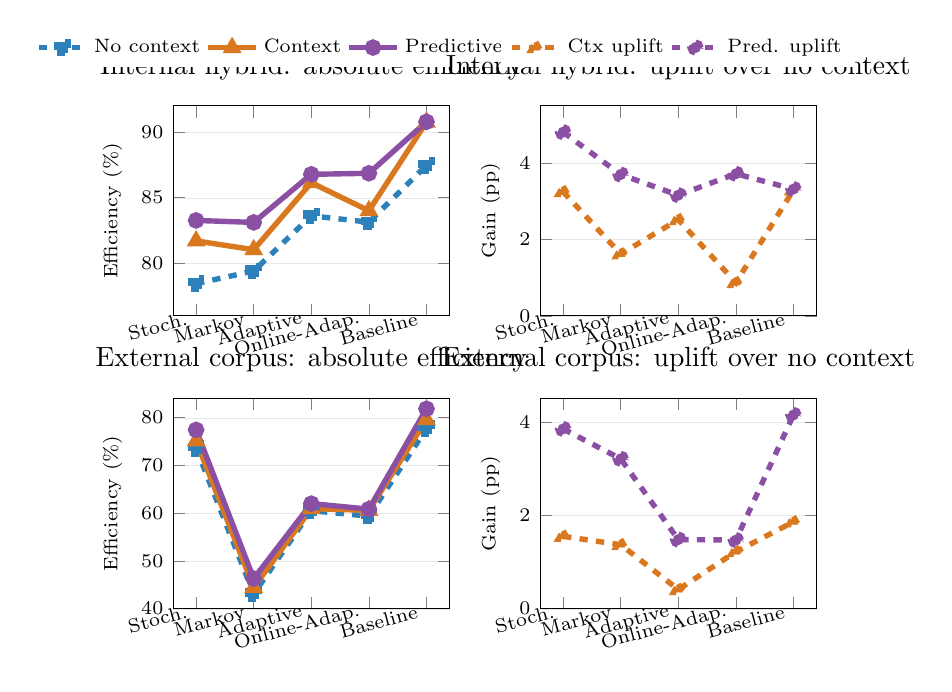
\begin{tikzpicture}
\begin{groupplot}[
group style={group size=2 by 2, horizontal sep=1.15cm, vertical sep=1.05cm},
width=0.42\textwidth,
height=4.25cm,
xtick={1,2,3,4,5},
xticklabels={Stoch.,Markov,Adaptive,Online-Adap.,Baseline},
xticklabel style={font=\scriptsize, rotate=15, anchor=east},
ymajorgrids=true,
grid style={line width=.1pt, draw=gray!18},
tick label style={font=\scriptsize},
label style={font=\scriptsize},
legend style={font=\scriptsize, draw=none, at={(0.5,1.18)}, anchor=south, legend columns=5},
every axis plot/.append style={line width=1.95pt},
every mark/.append style={scale=0.85}
]
\nextgroupplot[
title={Internal hybrid: absolute efficiency},
ylabel={Efficiency (\%)},
ymin=76, ymax=92
]
\addplot[color=phaseblue!85!black, mark=square*, dashed] coordinates {
  (1,78.46) (2,79.42) (3,83.62) (4,83.14) (5,87.46)
};
\addlegendentry{No context}
\addplot[color=phaseorange!95!black, mark=triangle*] coordinates {
  (1,81.71) (2,81.04) (3,86.14) (4,84.01) (5,90.76)
};
\addlegendentry{Context}
\addplot[color=phasepurple!90!black, mark=*] coordinates {
  (1,83.27) (2,83.12) (3,86.78) (4,86.86) (5,90.78)
};
\addlegendentry{Predictive context}

\nextgroupplot[
title={Internal hybrid: uplift over no context},
ylabel={Gain (pp)},
ymin=0, ymax=5.5
]
\addplot[color=phaseorange!95!black, mark=triangle*, dashed] coordinates {
  (1,3.25) (2,1.62) (3,2.52) (4,0.87) (5,3.30)
};
\addlegendentry{Ctx uplift}
\addplot[color=phasepurple!90!black, mark=*, dashed] coordinates {
  (1,4.81) (2,3.70) (3,3.16) (4,3.72) (5,3.32)
};
\addlegendentry{Pred. uplift}

\nextgroupplot[
title={External corpus: absolute efficiency},
ylabel={Efficiency (\%)},
ymin=40, ymax=84
]
\addplot[color=phaseblue!85!black, mark=square*, dashed] coordinates {
  (1,73.59) (2,43.09) (3,60.52) (4,59.38) (5,77.71)
};
\addplot[color=phaseorange!95!black, mark=triangle*] coordinates {
  (1,75.14) (2,44.46) (3,60.93) (4,60.60) (5,79.57)
};
\addplot[color=phasepurple!90!black, mark=*] coordinates {
  (1,77.44) (2,46.30) (3,62.00) (4,60.85) (5,81.86)
};

\nextgroupplot[
title={External corpus: uplift over no context},
ylabel={Gain (pp)},
ymin=0, ymax=4.5
]
\addplot[color=phaseorange!95!black, mark=triangle*, dashed] coordinates {
  (1,1.55) (2,1.37) (3,0.41) (4,1.22) (5,1.86)
};
\addplot[color=phasepurple!90!black, mark=*, dashed] coordinates {
  (1,3.85) (2,3.21) (3,1.48) (4,1.47) (5,4.15)
};
\end{groupplot}
\end{tikzpicture}
\caption{Quantum context-spectrum results decomposed into absolute performance and marginal uplift. The left column shows the absolute efficiency trajectories for no-context, contextual, and predictive-context families in the internal and external corpora. The right column shows how much contextual and predictive context improve over the corresponding no-context baseline in each scenario. This makes the scientific point explicit: richer context helps everywhere, but the size of the gain is scenario dependent and is usually largest for the predictive-context family.}
\label{fig:context_spectrum}
\end{figure*}

Figure~\ref{fig:context_spectrum} is more informative than the earlier version because it separates absolute routing quality from the incremental value of added context. The uplift panels show that predictive context is consistently the strongest improvement family, while the size of the gain varies materially by threat regime rather than remaining constant across scenarios.

\subsection{Clinical Preliminary Results}
The clinical side contributes preliminary evidence from the EQUITAS
bioinformatics source package. This evidence is not presented as final
patient-level validation; instead, it supplies a concrete diagnostic-relevant
case showing why context availability matters. In this setting, lower context
corresponds to structure prediction without thermodynamic/context-aware scoring,
while richer context corresponds to Nussinov/MFE feature augmentation,
fairness-aware Synthetic LowGC augmentation, and subgroup-aware EQUITAS auditing.

\begin{table*}[t]
\caption{Preliminary clinical results from the EQUITAS bioinformatics evidence package.}
\label{tab:clinical_prelim_results}
\centering
\small
\setlength{\tabcolsep}{5pt}
\begin{tabular}{p{0.07\textwidth}p{0.35\textwidth}p{0.26\textwidth}p{0.25\textwidth}}
\toprule
\textbf{Evidence source} & \textbf{Current quantitative signal} & \textbf{Why it matters} & \textbf{How it feeds this paper} \\
\midrule
EQUITAS corpus & dataset expanded from 10 to 20 RNA sequences, including 10 Synthetic LowGC sequences & makes clinical-like context gaps measurable in a controlled biomedical proxy task & informs the missingness and group-representation design of the planned simulator \\
Enhanced Nussinov tuning & Optuna search over 30 trials produced an optimized objective of 56.44 and mean predicted-pair output of 66.07 $\pm$ 46.36 & shows that richer structural context can materially change diagnostic-relevant prediction behavior & motivates comparing lower-context and richer-context decision policies \\
Context ablation & thermodynamic/context-aware scoring reported 61.36 $\pm$ 44.21 predicted pairs versus 14.96 $\pm$ 10.45 without that context & directly supports the rough draft's context-gain thesis in the clinical testbed & anchors the clinical side of the cross-testbed context-gain comparison \\
Fairness audit & post-augmentation mitigation achieved 6/6 algorithm compliance with the 80\% rule, DI ratios of 1.000, and +0.805 average DI improvement & demonstrates that representation/context repair can improve fairness indicators, not only utility & supplies preliminary fairness evidence before final sequential bandit experiments \\
\bottomrule
\end{tabular}
\end{table*}

\begin{table}[t]
\caption{Aggregate context-gain comparison across the two preliminary evidence bases.}
\label{tab:cross_testbed_context_gain}
\centering
\small
\setlength{\tabcolsep}{4pt}
\begin{tabular}{p{0.28\columnwidth}ccc}
\toprule
\textbf{Testbed} & \textbf{Lower ctx.} & \textbf{Richer ctx.} & \textbf{Gain} \\
\midrule
Quantum routing & 82.39\% & 86.13\% & +3.74 pp \\
Clinical bioinformatics & 14.96 pairs & 66.07 pairs & +51.11 pairs \\
\bottomrule
\end{tabular}
\end{table}

\begin{figure*}[t]
\centering
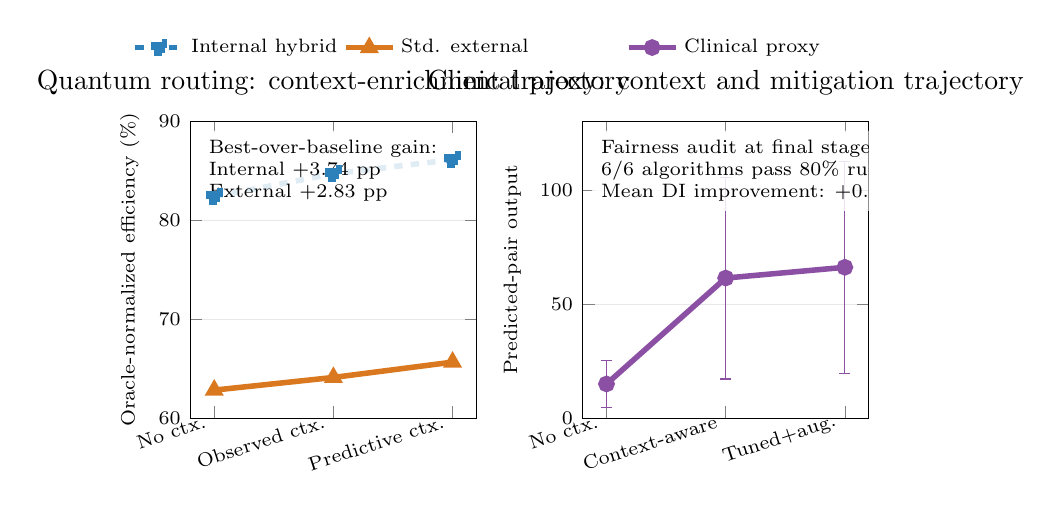
\begin{tikzpicture}
\begin{groupplot}[
group style={group size=2 by 1, horizontal sep=1.35cm},
width=0.43\textwidth,
height=5.35cm,
xtick=data,
xticklabel style={font=\scriptsize, rotate=18, anchor=east},
tick label style={font=\scriptsize},
label style={font=\scriptsize},
ymajorgrids=true,
grid style={line width=.1pt, draw=gray!18},
legend style={font=\scriptsize, draw=none, at={(0.5,1.18)}, anchor=south, legend columns=3},
every axis plot/.append style={line width=2pt},
every mark/.append style={scale=0.9}
]
\nextgroupplot[
title={Quantum routing: context-enrichment trajectory},
ylabel={Oracle-normalized efficiency (\%)},
symbolic x coords={No ctx.,Observed ctx.,Predictive ctx.},
ymin=60, ymax=90
]
\addplot[color=phaseblue!85!black, mark=square*, dashed] coordinates {
  (No ctx.,82.39) (Observed ctx.,84.70) (Predictive ctx.,86.13)
};
\addlegendentry{Internal hybrid}
\addplot[color=phaseorange!95!black, mark=triangle*] coordinates {
  (No ctx.,62.83) (Observed ctx.,64.11) (Predictive ctx.,65.66)
};
\addlegendentry{Std. external}
\node[anchor=north west, font=\scriptsize, align=left,
      fill=white, fill opacity=0.85, text opacity=1, rounded corners=2pt]
  at (rel axis cs:0.03,0.97)
  {Best-over-baseline gain:\\Internal +3.74 pp\\External +2.83 pp};

\nextgroupplot[
title={Clinical proxy: context and mitigation trajectory},
ylabel={Predicted-pair output},
symbolic x coords={No ctx.,Context-aware,Tuned+aug.},
ymin=0, ymax=130
]
\addplot[color=phasepurple!90!black, mark=*, error bars/.cd, y dir=both, y explicit] coordinates {
  (No ctx.,14.96) +- (0,10.45)
  (Context-aware,61.36) +- (0,44.21)
  (Tuned+aug.,66.07) +- (0,46.36)
};
\addlegendentry{Clinical proxy}
\node[anchor=north west, font=\scriptsize, align=left,
      fill=white, fill opacity=0.85, text opacity=1, rounded corners=2pt]
  at (rel axis cs:0.03,0.97)
  {Fairness audit at final stage:\\6/6 algorithms pass 80\% rule\\Mean DI improvement: +0.805};
\end{groupplot}
\end{tikzpicture}
\caption{Cross-testbed context-enrichment trajectories. The left panel shows that quantum-routing performance improves monotonically as the policy moves from no context to observed context to predictive context, with consistent gains in both the internal hybrid corpus and the standardized external corpus. The right panel separates two clinical effects that the previous normalized bar chart hid: restoring domain-relevant context produces the large primary gain (14.96 to 61.36 predicted pairs), while tuning and fairness-oriented augmentation provide a smaller secondary improvement (66.07 at the final stage) together with improved parity indicators. This presentation is more informative than a single normalized index because it distinguishes pure context recovery from later mitigation or refinement.}
\label{fig:cross_testbed_context_gain}
\end{figure*}

Figure~\ref{fig:cross_testbed_context_gain} provides a more scientific cross-testbed view than a single normalized bar chart. It shows that quantum gains are steady and incremental across context levels, whereas the clinical proxy is dominated by a large first-stage recovery when domain-relevant context is restored and then a smaller second-stage gain associated with tuning and fairness-aware augmentation.

\iffalse
\begin{figure}[t]
\centering
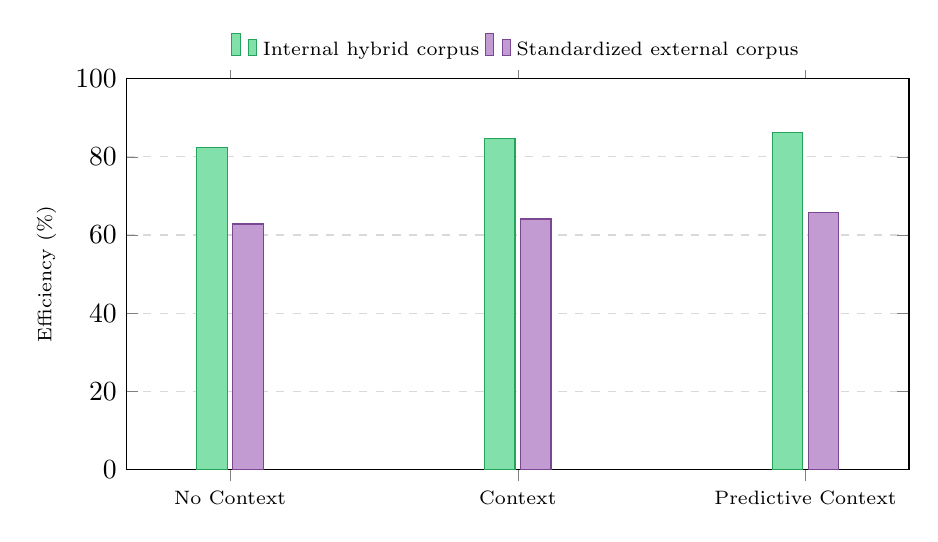
\begin{tikzpicture}
\begin{axis}[
    width=0.95\columnwidth,
    height=0.54\columnwidth,
    ybar,
    bar width=11pt,
    ymin=0, ymax=100,
    ylabel={Efficiency (\%)},
    symbolic x coords={No Context,Context,Predictive Context},
    xtick=data,
    xticklabel style={font=\scriptsize, align=center},
    ylabel style={font=\scriptsize},
    legend style={font=\scriptsize, at={(0.5,1.02)}, anchor=south, legend columns=2, draw=none},
    ymajorgrids=true,
    grid style={dashed,gray!30},
    enlarge x limits=0.18
]
\addplot[fill=phase2green!60, draw=phase2green!80!black] coordinates {
    (No Context,82.39)
    (Context,84.70)
    (Predictive Context,86.13)
};
\addplot[fill=phase4purple!60, draw=phase4purple!80!black] coordinates {
    (No Context,62.83)
    (Context,64.11)
    (Predictive Context,65.66)
};
\legend{Internal hybrid corpus,Standardized external corpus}
\end{axis}
\end{tikzpicture}
\caption{Preliminary result viewed as a context spectrum. Across both the
internal hybrid corpus and the standardized external corpus, richer context is
associated with higher Oracle-normalized efficiency: no-context baselines are
lowest, contextual policies improve on them, and predictive-context policies
perform best.}
\label{fig:context_spectrum}
\end{figure}
\fi

\begin{table}[t]
\caption{Current validation evidence and interpretation.}
\label{tab:validation}
\centering
\small
\begin{tabular}{p{0.38\columnwidth}p{0.52\columnwidth}}
\toprule
\textbf{Evidence} & \textbf{Interpretation} \\
\midrule
CRISP+ML quick pipeline runs & reviewer can execute the code artifact end-to-end \\
Stage unit tests pass & lifecycle stages have isolated behavior checks \\
Merge-check command passes & local validation path is ready for PR gating \\
Quantum execution paths documented & final experiments can start from notebook, local, or GCP workflows \\
State architecture documented & interrupted long-running tests can be resumed or audited \\
\bottomrule
\end{tabular}
\end{table}

Table~\ref{tab:validation} frames the current evidence conservatively. It
supports reproducibility and readiness, not final claims about which policy is
fairest. The final paper will replace or extend this table with empirical
curves, statistical summaries, and domain-specific fairness results.

Table~\ref{tab:prelim_results} makes the current evidence more concrete. The
rough draft can already report real quantum results because the project builds
on an existing validated experiment corpus and an associated manuscript. In the
standardized 4K/2K external corpus, the four inherited testbeds contribute
8,060 rows of model--scenario--allocator--scale evaluations. In the internal
hybrid corpus, the strongest current average efficiency belongs to
\texttt{iCPursuitNeuralUCB} (86.13\%), followed by
\texttt{CPursuitNeuralUCB} (84.70\%), \texttt{GNeuralUCB} (82.83\%), and
\texttt{EXPNeuralUCB} (81.95\%). These are meaningful preliminary results: they identify the current utility frontier
and expose which policy families are worth extending first.

Just as importantly, the current results can already be organized according to
the project's core scientific claim: \emph{context quality matters}. Rather
than treating the preliminary evidence as a list of algorithm names,
Table~\ref{tab:context_spectrum} and Figure~\ref{fig:context_spectrum} recast
the existing quantum framework work as evidence into a three-level spectrum. The no-context condition
captures reward-only or non-context baselines, the context condition captures
methods that use observed contextual structure, and the predictive-context
condition captures the informative or forecasting-aware extension. In both the
internal and external corpora, performance rises as the method family moves
from no context to context to predictive context. That pattern is exactly what
motivates our work extension: if richer context already improves utility,
the next question is whether fairness-aware and missingness-aware context
handling can also improve equity.

The external standardized corpus also shows that results vary by testbed
structure. Mean efficiencies for \texttt{iCPursuitNeuralUCB} are currently
about 74.34\% on Paper~2, 78.39\% on Paper~7, 73.95\% on Paper~8, and 42.54\%
on Paper~12. This matters for our work because it already suggests
that fairness conclusions should not be tied to a single network topology or
threat setting. A fairness-aware extension that appears successful in one
testbed but fails in another would still be a useful scientific finding.

From the standpoint of the rough-draft requirement, these results answer the
most important preliminary question: does the system already do something real
and measurable? Yes. The inherited quantum framework already executes correctly,
produces large validated datasets, distinguishes strong and weak model
families, and supports claims about robustness, efficiency, and configuration
effects. The new contribution of the final paper is to attach an explicit
fairness layer to those same data and test whether the best utility policies
also behave equitably under missing context.

The most important current result is that the research workflow has converged
into a coherent experiment plan. Earlier pieces of the semester work existed as
separate deliverables. This rough draft integrates those pieces into a single project narrative. The
implementation now has a reviewer-safe CRISP+ML path, a quantum-first execution
path, a state-management strategy, and a defined fairness layer. This reduces
the risk that final experiments will produce isolated performance numbers
without enough provenance to explain them.

The expected preliminary figures for the final report are also now specified.
For each scenario, the analysis will report reward or efficiency curves,
oracle gap, subgroup or flow-level disparity curves, and mitigation tradeoff
plots. For cross-domain transfer, the analysis will compare whether a
mitigation strategy that reduces missing-context disparity in one domain also
reduces it in the other. If transfer fails, that failure is still informative:
it would suggest that the shared framework is useful for diagnosing differences
between domains even when a single mitigation rule does not generalize.

\section{Future Work}
Next, the focus will be on completing the experimental contribution. First,
the quantum fairness adapter will connect evaluator and runner outputs to
service-equity metrics such as success-probability and latency gaps. This will
turn the existing quantum-routing performance infrastructure into a
fairness-aware analysis pipeline. Second, the clinical diagnostic simulator
will be implemented with controlled missingness, group-dependent measurement
noise, diagnostic action choices, and error outcomes. This simulator will allow
the project to test false-negative and false-positive gaps without relying on
sensitive patient records during development.

Third, at least one mitigation mechanism will be added and compared against
utility-only baselines. The initial priority is a simple fairness-regularized
or missingness-aware update rule that can be implemented in both domains.
Fourth, the same policy stack will be evaluated across both domains to test
whether fairness mechanisms transfer. Fifth, the final report will add full
results, plots, statistical discussion, and a stronger conclusion grounded ini
experimental evidence. The final analysis will also include a limitations
section discussing simulation validity, group-definition choices, and the
difference between fairness in a controlled testbed and fairness in deployment.

\section{Conclusion}
This semester established the foundation for a reproducible fairness-aware
contextual bandit project. The work completed so far includes a related-work
survey, a shared missing-context domain model, an approach and architecture
writeup, a cleaned code-review repository, documented notebook/local/GCP
execution paths, and a runnable CRISP+ML validation package. The project is positioned to move from design and infrastructure into final
experiments. Its expected impact is a practical framework for measuring and
mitigating fairness disparities in sequential decision systems where context
is incomplete, non-stationary, and unequally distributed across groups.

The next version of the paper will replace the current validation evidence with
complete experimental results. However, the structure needed for those results
is now in place: the literature gap is defined, the domain model is explicit,
the architecture is reproducible, the data contracts are identified, and the
ethical requirements are stated as part of the technical design. That makes the
remaining work a focused execution task.

\bibliographystyle{IEEEtran}
\bibliography{rough_draft_references}

\end{document}